\section{Introduction}

Testing is an essential part of any software development process. Although development of such test suites are hard and tedious, it saves time later in the development process to find bugs in the program. Software testers often want their testing framework to cover all the corner cases that exist in a program and localize possible bugs as much as possible. Unit test suite is one type of testing method that provide high level of localization but still test suite need to be critically designed to identify maximum number of bugs, if not all. 

Several techniques have been proposed to help test suites achieve high coverage. Mutation testing is one of such method. In mutation testing, a bug is deliberately introduced in the program. This bug is also called mutant and is often represented as a modification of operator that affect the semantics of the program. With each new mutant, a new program version is generated and tested using the provided test suite. For a mutated program, if a test in the test suite fails and that failing test case point to the mutated code then the test suite is capable of killing that mutant. If a test suite passes on a mutated program then the test suite lacks coverage and should be expanded so that it can kill the mutant.  This process is repeated for several version of mutated program where mutant exist in different locations. Test suite is believe to be of high quality if it kills all the mutants. Mutation testing helps software tester to improve their test suite coverage and its ability to find bugs.

Currently, several frameworks exist that provide support for mutation testing in different language like Java, C etc. Scala, on the other hand, does not have a source code level mutation testing framework. Inherently all the softwares developed on top of Scala or software that give Scala interface to users, does not offer mutation testing framework either, for example Spark. Spark is a data intensive scalable computing systems that is built on Scala and it expose its API to user in Scala. User written program in Spark include Scala code. These programs contain Spark API and user defined functions. Spark program can leverage a mutation testing framework to evaluate several fault and bug finding tools built for Spark.  

To meet all of these needs, we provide a configurable, flexible and target oriented mutation testing framework for Scala and Spark. This framework provides users an interface to configure user defined mutation operators and program locations to be mutated in case of Spark. Furthermore, it also enables user to apply probabilistic mutation on the program. Its flexible mutation operator mapping allows user to define a replacement criteria for an operator that is to be mutated. In the single run, our framework generates several version of the program, each with a single but different mutant. In the case of Spark applications, our framework only targets the user defined functions for mutations.

We have evaluated our framework on X different subject Scala programs and Y Spark programs. Our results show that we mutated W \% of files successfully, on average and generated compilable mutated source code in Q\% of the cases. Moreover, we show the efficacy of our mutation framework by reporting the number of test cases it fails.
The rest of the paper is organized as follows. Section 2 summarizes the related work that have been done in the past. Section 3 describes the architecture of our framework and step by step details of how it mutates a program. Section 4 presents the evaluation results from our experiments. 
\begin{figure*}[ht!]
\begin{center}
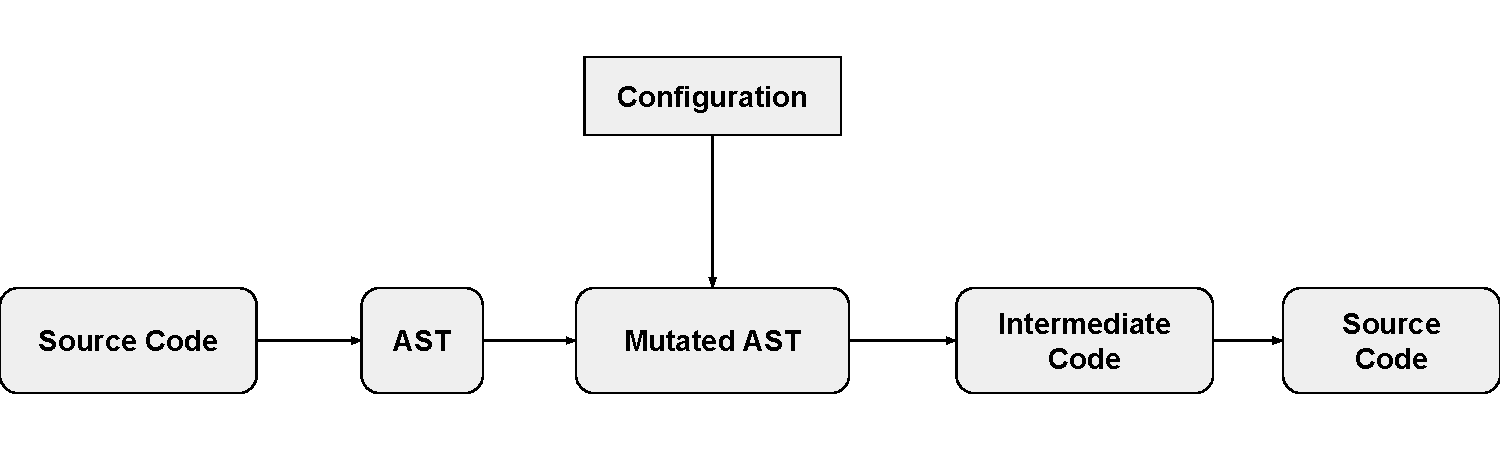
\includegraphics[width=0.8\textwidth]{image/flow}
\vspace{-1em}
   \caption{Mutation Framework Architecture}
   \vspace{-1.5em}
        \label{flow}
\end{center}
\end{figure*}
